\chapter{Implementierung am Beispiel der kommunalen Verwaltung}
\label{cha:implementierung}

\section{Konkretisierung der Problemstellung}
\begin{spacing}{1.5}

Die Nutzung von Zensusdaten in der öffentlichen Verwaltung stellt hohe Anforderungen an Datenschutz und Datensicherheit. Einerseits sind diese Daten äußerst wertvoll für analytische Zwecke, wie die Planung von Infrastrukturprojekten, die Bereitstellung von Sozialdiensten und die Verbesserung der öffentlichen Sicherheit. Andererseits müssen strenge Datenschutzrichtlinien eingehalten werden, um die Vertraulichkeit und Integrität der sensiblen Informationen zu gewährleisten.

Im Rahmen dieser Arbeit wird die Problematik der Nutzung realer Zensusdaten für Forschungszwecke beleuchtet. Traditionelle Methoden zur Anonymisierung stoßen häufig an ihre Grenzen, da sie nicht immer vollständig vor Re-Identifikationsrisiken schützen können. Dies führt zu einem Spannungsfeld zwischen der Notwendigkeit, detaillierte Daten zu verwenden, und der Pflicht, die Privatsphäre der Betroffenen zu schützen.

Die Lösung dieses Dilemmas könnte in der Verwendung synthetischer Daten liegen. Diese bieten die Möglichkeit, realistische, aber dennoch fiktive Daten zu generieren, die statistisch und strukturell den Originaldaten ähneln, jedoch keine direkten Rückschlüsse auf individuelle Personen zulassen. Die Frage, ob synthetische Zensusdaten eine praktikable Alternative zu realen Zensusdaten darstellen können, wird im weiteren Verlauf dieser Arbeit genauer untersucht.

\end{spacing}
\section{Auswahl und Spezifikation des Synthesizer-Tools}
\label{sec:synthesizer-tool-selection}
\begin{spacing}{1.5}

Für das Forschungsziel dieser Arbeit wurde die open-source Python-Library \textit{Synthetic Data Vault} (\acrshort{sdv}) ausgewählt \cite{synthetic_data_vault_2016}. \acrshort{sdv} bietet eine breite Palette an generativen Modellen wie Gaussian Copula, \acrshort{ctgan} und CopulaGAN, die qualitativ hochwertige synthetische Daten erzeugen können. Als Synthesizer wurde der \textit{CTGANSynthesizer} von \acrshort{sdv} verwendet. Dieses Modell nutzt \acrshort{gan}s, speziell das Conditional Tabular GAN-Modell (\acrshort{ctgan}), wie es von Xu et al. beschrieben wurde \cite{xu_modeling_2019}.

Es ist jedoch anzumerken, dass kommerzielle Lösungen wie Gretel oder Mostly AI aktuell noch überlegen sind \cite[60]{hradec_multipurpose_2022}, insbesondere hinsichtlich der Benutzerfreundlichkeit und der Tiefe automatisch generierter Reports und Analysen. Vor allem, wenn es darum geht, komplexere Tabellen mit einer Vielzahl von Einschränkungen, hoch kardinalen kategorialen Variablen und diskreten Daten zu verarbeiten, stoßen Open-Source-Lösungen an ihre Grenzen \cite[57]{hradec_multipurpose_2022}. Dennoch entwickelt sich das Feld der Open-Source-Lösungen schnell weiter, und es ist zu erwarten, dass in naher Zukunft wettbewerbsfähige Alternativen verfügbar sein werden.

Trotz der aktuellen Überlegenheit kommerzieller Lösungen genügt \acrshort{sdv} den Anforderungen dieser Studie. Es bietet die notwendige Datenqualität und Flexibilität, um die Synthesemethoden an die spezifischen Gegebenheiten der Zensusdaten anzupassen. Zudem stellt \acrshort{sdv} eine günstige Lösung dar, die ohne Lizenzkosten auskommt und somit besser in das Budget dieser Forschungsarbeit passt.

\end{spacing}
\section{Generierung synthetischer Zensusdaten}
\begin{spacing}{1.5}

Der zugrunde liegende Datensatz, der Census Income Dataset, wird von \acrshort{sdv} bereitgestellt und basiert auf dem ursprünglichen Census Income Dataset des UCI Machine Learning Repository \cite{misc_adult_2}. Die darin enthaltenen Daten wurden 1994 durch das United States Census Bureau erhoben und umfassen demografische und sozioökonomische Informationen von 32.561 Personen. In der Forschung wird dieser Datensatz häufig hergenommen, um Kausalitäten zu untersuchen, meist hinsichtlich der Frage, wovon das Einkommens einer Person abhängt\footnote{So etwa \cite{lazar_income_2004, islam_rana_investigation_2024, chakrabarty_statistical_2018}}. Die \acrshort{sdv}-Version dieses Datensatzes\footnote{Datensatz erreichbar unter: \url{https://sdv-demo-datasets.s3.amazonaws.com/SINGLE_TABLE/census_extended.zip}} erweitert jenen Ursprungsdatensatz um zusätzliche Spalten, einschließlich eines Quasi-Identifikators wie beispielsweise einer Adresse -- wobei diese fiktiv ist. Der Datensatz eignet sich als Beispiel für die Kommunalverwaltung aufgrund seiner umfassenden und vielfältigen Attribute, die typische Verwaltungsdaten widerspiegeln. So enthält er nicht nur demografische Informationen wie Alter, Geschlecht und Bildung, sondern auch sozioökonomische Merkmale wie Beruf, Arbeitszeit und Einkommensstufe.

\begin{table}[!htb]
    \centering\footnotesize
    \begin{tabular}{llllll}
        \toprule
        \\[-0.7em]
        age & workclass & education & race & income & address \\
        \\[-0.9em]
        \midrule
        \\[-0.7em]
        39 & State-gov & Bachelors & White & <=50K & 058 Wilson Inlet Apt. 470 Lake ...\\
        50 & Self-emp-not-inc & Bachelors & White & >50K & 9915 Andrew Road Ericashire ...\\
        38 & Private & HS-grad & White & <=50K & 4656 Tammy Terrace East Tonya ...\\
        53 & Private & 11th & Black & <=50K & 503 Danielle Dam South Melissa ...\\
        \\[-0.9em]
        \bottomrule
    \end{tabular}
    \caption[Auszug des verwendeten Datensatzes mit ausgewählten Spalten]{Auszug des verwendeten Datensatzes mit ausgewählten Spalten\footnotemark}
    \label{tab:census-data-sample}
\end{table}
\footnotetext{Eigene Darstellung}

\begin{figure}[ht]
\begin{center}
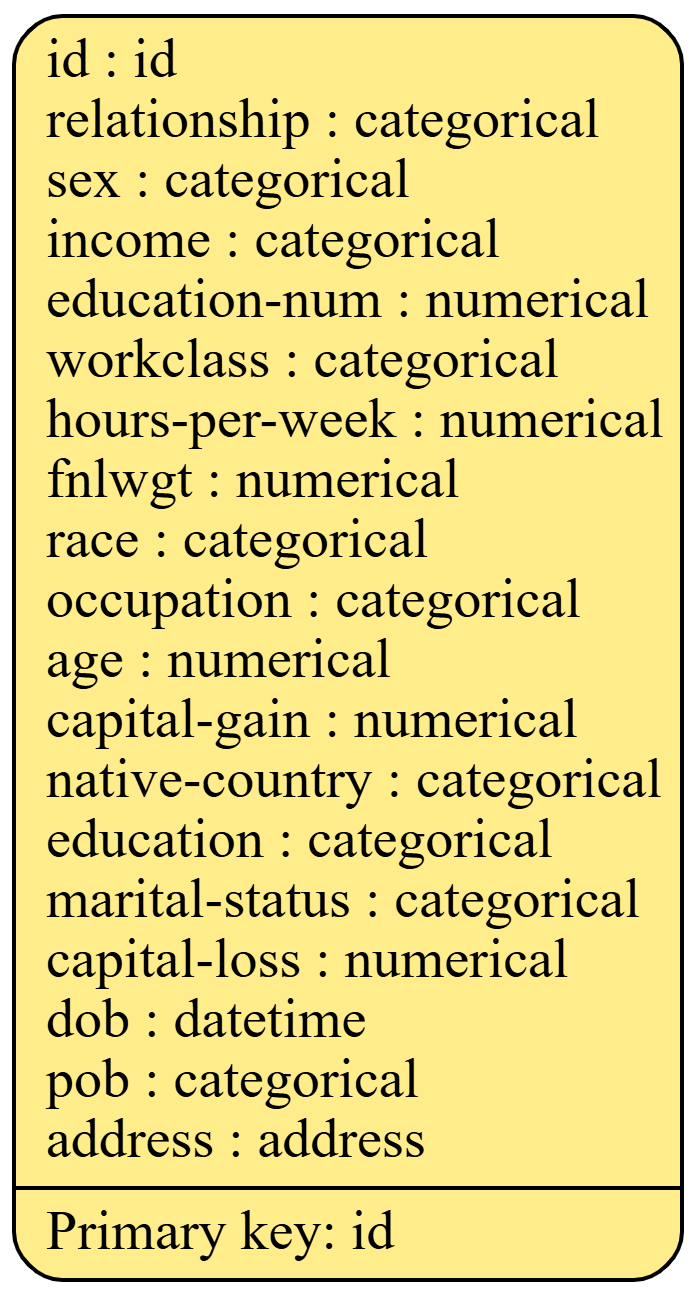
\includegraphics[width=0.24\textwidth]{img/metadata.png}
\caption[Beschreibung der Attribute inkl. Datentypen und Primärschlüssel]{Beschreibung der Attribute inkl. Datentypen und Primärschlüssel}
\label{fig:metadata}
\end{center}
\end{figure}

Nachdem die Metadaten (vgl. Abbildung \ref{fig:metadata}) festgelegt wurden, wird der im vorherigen Abschnitt \ref{sec:synthesizer-tool-selection} behandelte CTGANSynthesizer erstellt (vgl. Anhang 2). Mittels maschinellen Lernens wird der Synthesizer anschließend auf den gesamten 32.561 Einträgen trainiert. Unter Verwendung einer Tesla GPU 4\footnote{Bereitgestellt durch Google Colabs Compute Engine-Back-End} hat das Training 12 Minuten gedauert. Abschließend kann mithilfe der sample-Methode eine beliebige Anzahl an synthetischen Daten erzeugt werden, welche es im nächsten Kapitel zu evaluieren gilt.

\end{spacing}